\chapter*{Основная часть}
\label{cha:analysis}

\setcounter{section}{0} % Устанавливаем начальное значение для раздела
\renewcommand\thesection{\arabic{section}} % Устанавливаем формат номера раздела как просто цифру

\section{Теоретическая часть}

Метод Гаусса является прямым методом решения СЛАУ, который заключается в последовательном исключении переменных. Он трансформирует исходную систему уравнений в эквивалентную систему, матрица которой является верхней треугольной. Эта трансформация достигается путем выполнения элементарных преобразований над строками расширенной матрицы $[A|b]$, где $A$ - матрица коэффициентов, а $b$ - вектор свободных членов. Подробное описание метода Гаусса можно найти, например, в \cite{krivosonova2005numerical}.

\subsection*{Элементарные преобразования строк}
Элементарные преобразования строк, которые применяются в методе Гаусса, включают в себя:
\begin{itemize}
    \item Перестановка двух строк: $R_i \leftrightarrow R_j$
    \item Умножение строки на ненулевую константу: $R_i \rightarrow \lambda R_i$, где $\lambda \ne 0$
    \item Прибавление к одной строке другой строки, умноженной на константу: $R_i \rightarrow R_i + \lambda R_j$
\end{itemize}

\subsection*{Описание метода Гаусса с выбором ведущего элемента по строке}

Рассмотрим систему линейных уравнений $Ax = b$, где $A$ - матрица размера $n \times n$, $x$ - вектор неизвестных, и $b$ - вектор свободных членов.

\begin{enumerate}
    \item \textbf{Составление расширенной матрицы:} формируем расширенную матрицу $[A|b]$.

    \item \textbf{Прямой ход (исключение переменных):}
        Для каждого столбца $k$ (от 1 до $n$):
        \begin{enumerate}
            \item \textbf{Выбор ведущего элемента (по строке):}
               Находим индекс $p$ такой, что
               \begin{equation}
                  |a_{pk}| = \max_{k \leq i \leq n} |a_{ik}|
                   \label{eq:leading_elem}
               \end{equation}
               Здесь $a_{ik}$ - элемент в $i$-й строке и $k$-м столбце текущей матрицы. Индекс $p$ указывает на строку с наибольшим по модулю элементом в $k$-м столбце, начиная с $k$-ой строки.

           \item \textbf{Перестановка строк (если необходимо):}
                Если $p \neq k$, то меняем местами строки $k$ и $p$:
                \[
                   R_k \leftrightarrow R_p
                \]
            Это обеспечивает, что на диагонали будет элемент с наибольшим абсолютным значением в текущем столбце.

            \item \textbf{Нормализация строки:} делим $k$-ую строку на ведущий элемент $a_{kk}$
                \[
                    R_k \rightarrow \frac{1}{a_{kk}} R_k
                \]
               Это приводит к тому, что элемент на диагонали становится равным 1.

            \item \textbf{Исключение переменных:} для каждой строки $i$ ($k<i \leq n$), вычитаем из нее строку $k$, умноженную на $a_{ik}$:
                \[
                   R_i \rightarrow R_i - a_{ik} R_k
                \]
                Эта операция делает все элементы в $k$-м столбце ниже $k$-й строки равными 0.
        \end{enumerate}

    \item \textbf{Обратный ход (нахождение решения):}
        После прямого хода мы имеем систему $Ux = c$, где $U$ - верхняя треугольная матрица. Теперь находим решение $x_i$ начиная с последнего $x_n$:
           \begin{equation}
               x_i = c_i - \sum_{j=i+1}^n u_{ij} x_j \quad \text{для} \quad i = n-1, n-2, ..., 0
                \label{eq:back_substitution}
            \end{equation}
         где $c_i$ это элементы вектора $c$, а $u_{ij}$ это элементы матрицы $U$ \cite{isaev2011methods}.
\end{enumerate}

\subsection*{Выбор ведущего элемента}
Выбор ведущего элемента необходим для минимизации ошибок округления, возникающих при работе с числами с плавающей точкой.  Без выбора ведущего элемента, если на диагонали матрицы окажется малое число, операция деления в шаге 3 может привести к значительному увеличению ошибок округления. В свою очередь это повлияет на результат исключения переменных. Выбор ведущего элемента по строке позволяет выбирать наибольшее (по модулю) число в текущем столбце в качестве диагонального элемента, что делает процесс вычислений более устойчивым и точным \cite{kolobov2008}.


\newpage


\section{Реализация}

Реализация метода Гаусса с выбором ведущего элемента по строке была выполнена на языке Python. Программный код представлен ниже:


\begin{lstlisting}[caption={Метод Гаусса с выбором ведущего элемента по строке на языке Python}]
import numpy as np
import matplotlib.pyplot as plt


def solve_with_row_main_elem_choice(A, b):
    matrix = np.hstack((A, b.reshape(-1, 1)))
    n = len(b)

    max_indexes_order = []
    answers = np.zeros(n)

    iters = 0

    for step in range(n):
        max_index = np.argmax(np.abs(matrix[step:, step])) + step
        max_elem = matrix[max_index, step]

        if max_elem == 0:
            raise ValueError("Matrix is degenerative.")

        if max_index != step:
            matrix[[step, max_index]] = matrix[[max_index, step]]

        matrix[step] = matrix[step] / max_elem

        iters += 1

        for i in range(step + 1, n):
            matrix[i] -= matrix[step] * matrix[i, step]
            iters += 1

        max_indexes_order.append(step)

    for i in range(n - 1, -1, -1):
        answers[i] = matrix[i, -1] - np.dot(matrix[i, i + 1:n], answers[i + 1:n])
        iters += 1

    return answers, iters


sizes = range(2, 100, 5)
iterations = []
times = []
errors = []

for size in sizes:
    A = np.random.rand(size, size) * 10
    b = np.random.rand(size) * 10
    x_gauss, iteration_count = solve_with_row_main_elem_choice(A, b)
    x_exact = np.linalg.solve(A, b)

    error = np.linalg.norm(x_gauss - x_exact)

    iterations.append(iteration_count)
    errors.append(error)


plt.figure(figsize=(8, 5))
plt.plot(sizes, iterations, label="Number of iterations", marker="o")
plt.xlabel("Size of matrix")
plt.ylabel("Number of iterations")
plt.title("Dependence of the number of iterations on the dimension of the matrix")
plt.grid(True)
plt.legend()
plt.tight_layout()
plt.show()

plt.figure(figsize=(8, 5))
plt.plot(sizes, errors, label="Error", marker="o", color="r")
plt.xlabel("Size of matrix")
plt.ylabel("Number of iterations")
plt.title("The dependence of the error on the dimension of the matrix")
plt.grid(True)
plt.legend()
plt.tight_layout()
plt.show()
\end{lstlisting}


\section{Экспериментальные исследования}

\subsection*{Зависимость количества операций от размерности матрицы}
На рисунке \ref{fig:iterations} показана зависимость количества операций от размерности матрицы. Видно, что количество операций растет кубически с увеличением размера матрицы, что соответствует теоретическим оценкам сложности метода Гаусса.

\begin{figure}
  \centering
  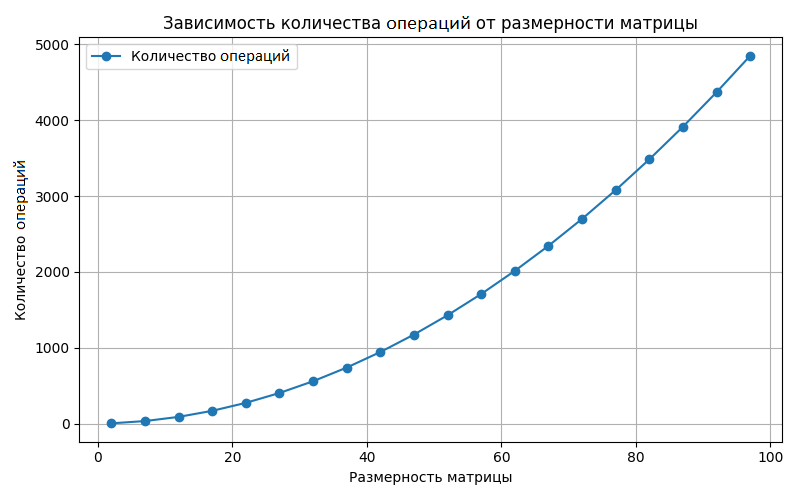
\includegraphics[width=\textwidth, height=9cm]{figures/1.png}
  \caption{Зависимость количества операций от размерности матрицы}
  \label{fig:iterations}
\end{figure}

\subsection*{Зависимость погрешности от размерности матрицы}

На рисунке \ref{fig:errors} представлена зависимость погрешности решения от размерности матрицы. Анализ графика показывает, что погрешность имеет сложную, нелинейную структуру, не демонстрируя ожидаемого монотонного роста. При малых размерностях погрешность минимальна, но наблюдается резкий выброс в районе размерности 30-35. Далее следуют колебания погрешности, а при больших размерностях (после 80) проявляется тенденция к её росту. Это указывает на то, что метод Гаусса с выбором ведущего элемента, хотя и устойчив в целом, подвержен ошибкам округления, зависящим как от размера, так и от структуры матрицы.

\begin{figure}
  \centering
  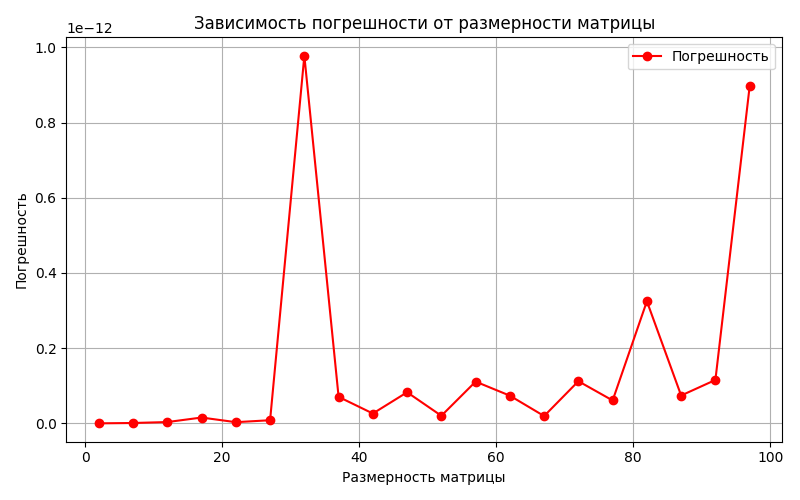
\includegraphics[width=\textwidth, height=9cm]{figures/2.png}
  \caption{Зависимость погрешности от размерности матрицы}
  \label{fig:errors}
\end{figure}

